% Full instructions available at:
% https://github.com/elauksap/focus-beamertheme

\documentclass{beamer}
\usetheme[numbering=progressbar]{focus}
\usepackage{tikz}
\usetikzlibrary{positioning}
\usetikzlibrary{shapes,arrows}
\usepackage{transparent}
\usepackage{fancyvrb}
\usepackage{listings}
\definecolor{main}{RGB}{47, 161, 219}
%\definecolor{textcolor}{RGB}{128, 128, 128}
\definecolor{background}{RGB}{240, 247, 255}
\definecolor{textcolor}{RGB}{85, 87, 83}
\title{D4 Project}
\subtitle{Open and collaborative network monitoring}
\author{Alexandre Dulaunoy - Sami Mokaddem}
\titlegraphic{
\includegraphics[scale=0.20]{d4-logo.pdf}}
\institute{Team CIRCL \\ \url{https://www.d4-project.org/}}
\date{20190207}

\begin{document}
    \begin{frame}
        \maketitle
    \end{frame}

\begin{frame}
        \frametitle{Problem statement}
        \begin{itemize}
                \item CSIRTs (or private organisations) build their {\bf own honeypot, honeynet or blackhole monitoring network}
                \item Designing, managing and operating such infrastructure is a tedious and resource intensive task
                \item {\bf Automatic sharing} between monitoring networks from different organisations is missing
                \item Sensors and processing are often seen as blackbox or difficult to audit

        \end{itemize}
\end{frame}


\begin{frame}
 \frametitle{Objective}
 \begin{itemize}
         \item Based on our experience with MISP\footnote{\url{https://github.com/MISP/MISP}} where sharing played an important role, we transpose
                 the model in D4 project
         \item Keeping the protocol and code base {\bf simple and minimal}
         \item Allowing every organisation to {\bf control and audit their own sensor network}
         \item Extending D4 or {\bf encapsulating legacy monitoring protocols} must be as simple as possible
         \item Ensuring that the sensor server has {\bf no control on the sensor} (unidirectional streaming)
         \item Don't force users to use dedicated sensors and allow {\bf flexibility of sensor support} (software, hardware, virtual)

 \end{itemize}
\end{frame}

\begin{frame}
        \frametitle{(short) History}
 \begin{itemize}
        \item D4 Project (co-funded under INEA CEF EU program) started - 1st November 2018
        \item D4 encapsulation protocol version 1 published  - 1st December 2018
        \item v0.1 release of the D4 core\footnote{\url{https://www.github.com/D4-project/d4-core}} including a server and simple D4 C client - 21st January 2018
        \item First version of a golang D4 client\footnote{\url{https://www.github.com/D4-project/d4-goclient/}} running on ARM, MIPS, PPC and x86 - January 2018
 \end{itemize}
\end{frame}

\begin{frame}
\frametitle{D4 Overview}
        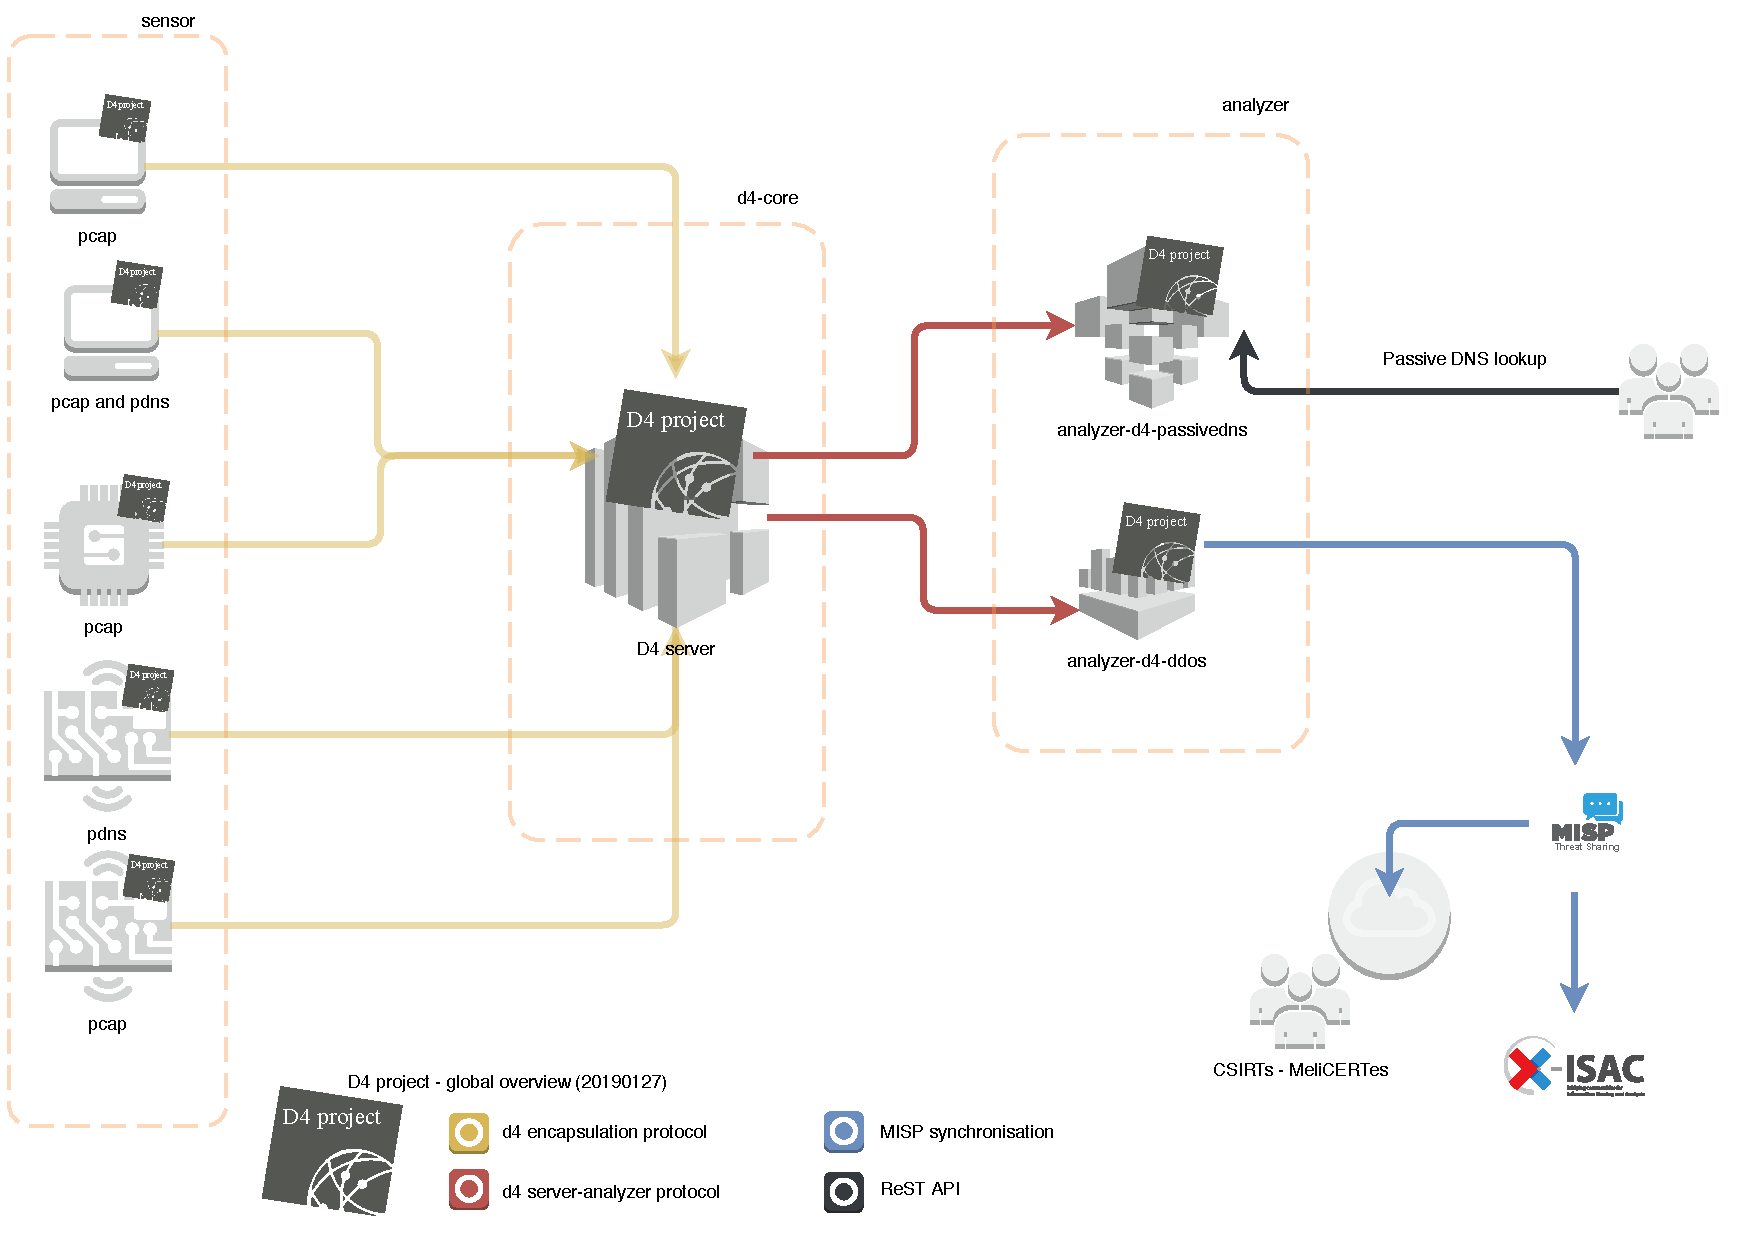
\includegraphics[scale=0.38]{d4-overview.pdf}
\end{frame}

\begin{frame}
        \frametitle{Roadmap (next 2 months)}
        \begin{itemize}
                \item Passive DNS analyzer (alpha version released)
                \item Passive SSL collector and analyzer
                \item Backscatter DDoS traffic analyzer
                \item {\bf Default server} (blackhole monitoring or Passive DNS collector) at CIRCL for organisations willing to contribute without running their own D4 server
        \end{itemize}
\end{frame}


\begin{frame}
        \frametitle{D4 encapsulation protocol}
        \includegraphics[scale=0.38]{d4-protocol-encapsulation.png}
\end{frame}

\begin{frame}
    \frametitle{D4 Header}
    \begin{tabular}{|l|l|l|}
        \hline
        Name & 	bit size&  	Description\\
        \hline
        version &	uint 8 &	Version of the header \\
        type 	& uint 8   &	Data encapsulated type\\
        uuid 	& uint 128 & 	Sensor UUID\\
        timestamp &  	uint 64 &	Encapsulation time\\
        hmac 	& uint 256 &	Authentication header (HMAC-SHA-256-128)\\
        size 	& uint 32 	& Payload size\\
        \hline
    \end{tabular}
\end{frame}


\begin{frame}
    \frametitle{D4 Header}
    \framesubtitle{Types}
        \begin{tabular}{|l|l|}
            \hline
            Type &	Description\\
            \hline
            0 	& Reserved\\
            1 	& pcap (libpcap 2.4)\\
            2 	& meta header (JSON)\\
            3 	& generic log line\\
            4 	& dnscap output\\
            5 	& pcapng (diagnostic)\\
            6 	& generic NDJSON or JSON Lines\\
            7 	& generic YAF (Yet Another Flowmeter)\\
            8  	& passivedns CSV stream\\
            254 &	type defined by meta header (type 2)\\
            \hline
        \end{tabular}
\end{frame}

\begin{frame}
    \frametitle{D4 meta header}
    \framesubtitle{Meta types}
    \small
    \begin{lstlisting}
{
  "type": "ja3-jl",
  "encoding": "utf-8",
  "tags": [
    "tlp:white"
  ],
  "misp:org": "5b642239-4db4-4580-adf4-4ebd950d210f"
}
\end{lstlisting}

\end{frame}


\begin{frame}
        \frametitle{}
{\center Use-case: migrating a legacy network capture model into a D4 network sensor
}
\end{frame}

\begin{frame}
\frametitle{Remote network capture}
    CIRCL operated honeybot for multiple years using a simple model of remote network capture.
    \begin{definition}[Principle]
        \begin{itemize}
            \item KISS (Keep it simple stupid) - Unix-like
            \item Linux \& OpenBSD operating systems
        \end{itemize}
    \end{definition}

    \begin{block}{Sensor}
    \lstset{%
        language=bash,
        backgroundcolor=\color{gray!25},
        basicstyle=\ttfamily,
        breaklines=true,
        columns=fullflexible
    }
    \begin{lstlisting}
tcpdump -l -s 65535 -n -i vr0 -w - '( not port $PORT and not host $HOST )' | socat - OPENSSL-CONNECT:$COLLECTOR:$PORT,cert=/etc/openssl/client.pem,cafile=/etc/openssl/ca.crt,verify=1
\end{lstlisting}


    \end{block}
\end{frame}

\begin{frame}
    \frametitle{Remote network capture}
    \begin{block}{Limitations}
        \begin{itemize}
            \item Scalability $\to$ one port per client
            \item Identification and registration of the client
            \item Integrity of the data
        \end{itemize}
    \end{block}

    \begin{block}{Multiplexing streams in D4}
        \begin{itemize}
            \item Inspired by the unix command {\tt tee}
            \item Read from standard input
            \item Add the d4 header
            \item Write it on standard output
        \end{itemize}
    \end{block}
\end{frame}


\begin{frame}
    \frametitle{Remote network capture with D4}
    \frametitle{Using D4 native client}
      \lstset{%
        language=bash,
        backgroundcolor=\color{gray!25},
        basicstyle=\ttfamily,
        breaklines=true,
        columns=fullflexible
    }
    \begin{lstlisting}
tcpdump -n -s0 -w - | ./d4 -c ./conf | socat - OPENSSL-CONNECT:$D4-SERVER-IP-ADDRESS:$PORT,verify=1
\end{lstlisting}


\begin{block}{Configuration directory}
    \begin{tabular}{l|l}
        Parameter & Explanation\\
        \hline
        type & see D4 Header slide\\
        source & standard input\\
        key & HMAC key\\
        uuid & Identifier of the sensor\\
        version &  version of the sensor\\
        destination & standard output\\
        snaplen & length of data being read \& written\\
    \end{tabular}
\end{block}
\end{frame}


\end{document}
